\section{Lubrificazione e Manutenzione}
\subsection{Lubrificazione}
Al termine dello studio di progettazione si prosegue spostando l’attenzione su uno degli aspetti di fondamentale importanza durante il funzionamento del compressore (come nella maggior parte dei sistemi meccanici che prevedono accoppiamenti), ovvero la lubrificazione.\\
L’interposizione di un agente liquido viscoso (olio) fra due superfici a contatto consente infatti di abbattere l’entità degli attriti, preservando l’integrità e prolungando la vita utile dei due elementi in moto relativo, riducendone inoltre le temperature nelle zone di collegamento.\\
\\
Nella macchina operatrice in esame la lubrificazione delle parti mobili avviene per “sbattimento”. Grazie alla presenza di una protuberanza nella parte inferiore della biella, che durante la rotazione della manovella impatta (in gergo “si tuffa”) ciclicamente l’olio contenuto nel carter, il lubrificante viene proiettato violentemente in tutte le direzioni, facendogli raggiungere, anche mediante condotti ricavati nei vari membri, tutte le superfici interessate. \\
Le zone di contatto del manovellismo di spinta che devono essere necessariamente raggiunte dal lubrificante sono:
\begin{itemize}
    \item Superficie di contatto fra camicia del cilindro e parete esterna del pistone.
    \item Contatti interni dei cuscinetti di banco dell’albero a gomiti (corpi volventi e piste).
    \item Accoppiamento piede di biella e spinotto. In questa superficie la penetrazione dell’olio è favorita dalla presenza di un imbuto nella parte superiore della biella, come mostrato in Fig.\ref{fig:LubrificazionePiedeBiella} .
    \item Superficie di interfaccia fra testa di biella e manovella dell’albero a gomiti. In questa zona la lubrificazione è garantita dalla presenza di un condotto appositamente realizzato per convogliare l’olio dalla parte inferiore dello stelo della biella verso la superficie di strisciamento Fig.\ref{fig:LubrificazioneTestaBiella} .
\end{itemize}
\begin{figure}[h]
    \centering
    \includegraphics[scale=0.3]{Immagini/LubrificazionePiedeBiella.png}
    \caption{Dettaglio lubrificazione piede di biella}
    \label{fig:LubrificazionePiedeBiella}
\end{figure}
\begin{figure}[h]
    \centering
    \includegraphics[scale=0.3]{Immagini/LubrificazioneTestaBiella.png}
    \caption{Dettaglio lubrificazione testa di biella}
    \label{fig:LubrificazioneTestaBiella}
\end{figure}
\subsection{Malfunzionamento e rottura della biella}
L’assenza di un' adeguata lubrificazione è sicuramente uno dei principali motivi che può portare a malfunzionamenti, usura precoce e, nel peggiore dei casi, anche alla rottura della macchina. \\
La condizione più critica, sia per compressori che per motori a pistoni, si localizza indubbiamente nella superficie di contatto fra testa di biella e manovella, dove i moti relativi sono più rilevanti e si è impossibilitati nell’utilizzare cuscinetti volventi. Nel caso del compressore in esame inoltre è assente la classica bronzina che si può trovare nelle macchine alternative veloci, per tale motivo ne risulta una criticità inevitabilmente amplificata. \\
Le pressioni di contatto su questa superficie devono infatti essere sufficientemente contenute, soprattutto perché ad essere in contatto sono due materiali con una sostanziale differenza in termini di durezza superficiale. La Ghisa GS-500 da noi considerata, infatti, ha durezza Brinell nell’ordine dei 200-240 HB a differenza dell’alluminio 201-T6 che si ferma “solo” a 95-110 HB. Ne consegue che durante il normale strisciamento della manovella all’interno della biella, quest’ultima subirà fenomeni di microerosione superficiale, che nel tempo possono portare a danneggiamenti e a depositi di materiale metallico.\\
Il risultato di questo processo è facilmente individuabile nella Fig.\ref{fig:SuperficiBiellaManovella} dove sono confrontate le morfologie superficiali dell’interno della testa di biella e della manovella su cui essa era impegnata. Si può notare difatti una maggior scalfitura della prima piuttosto che della seconda, che sembra pressoché ancora in condizioni simili all’originale. \\
\begin{figure}[h]
    \centering
    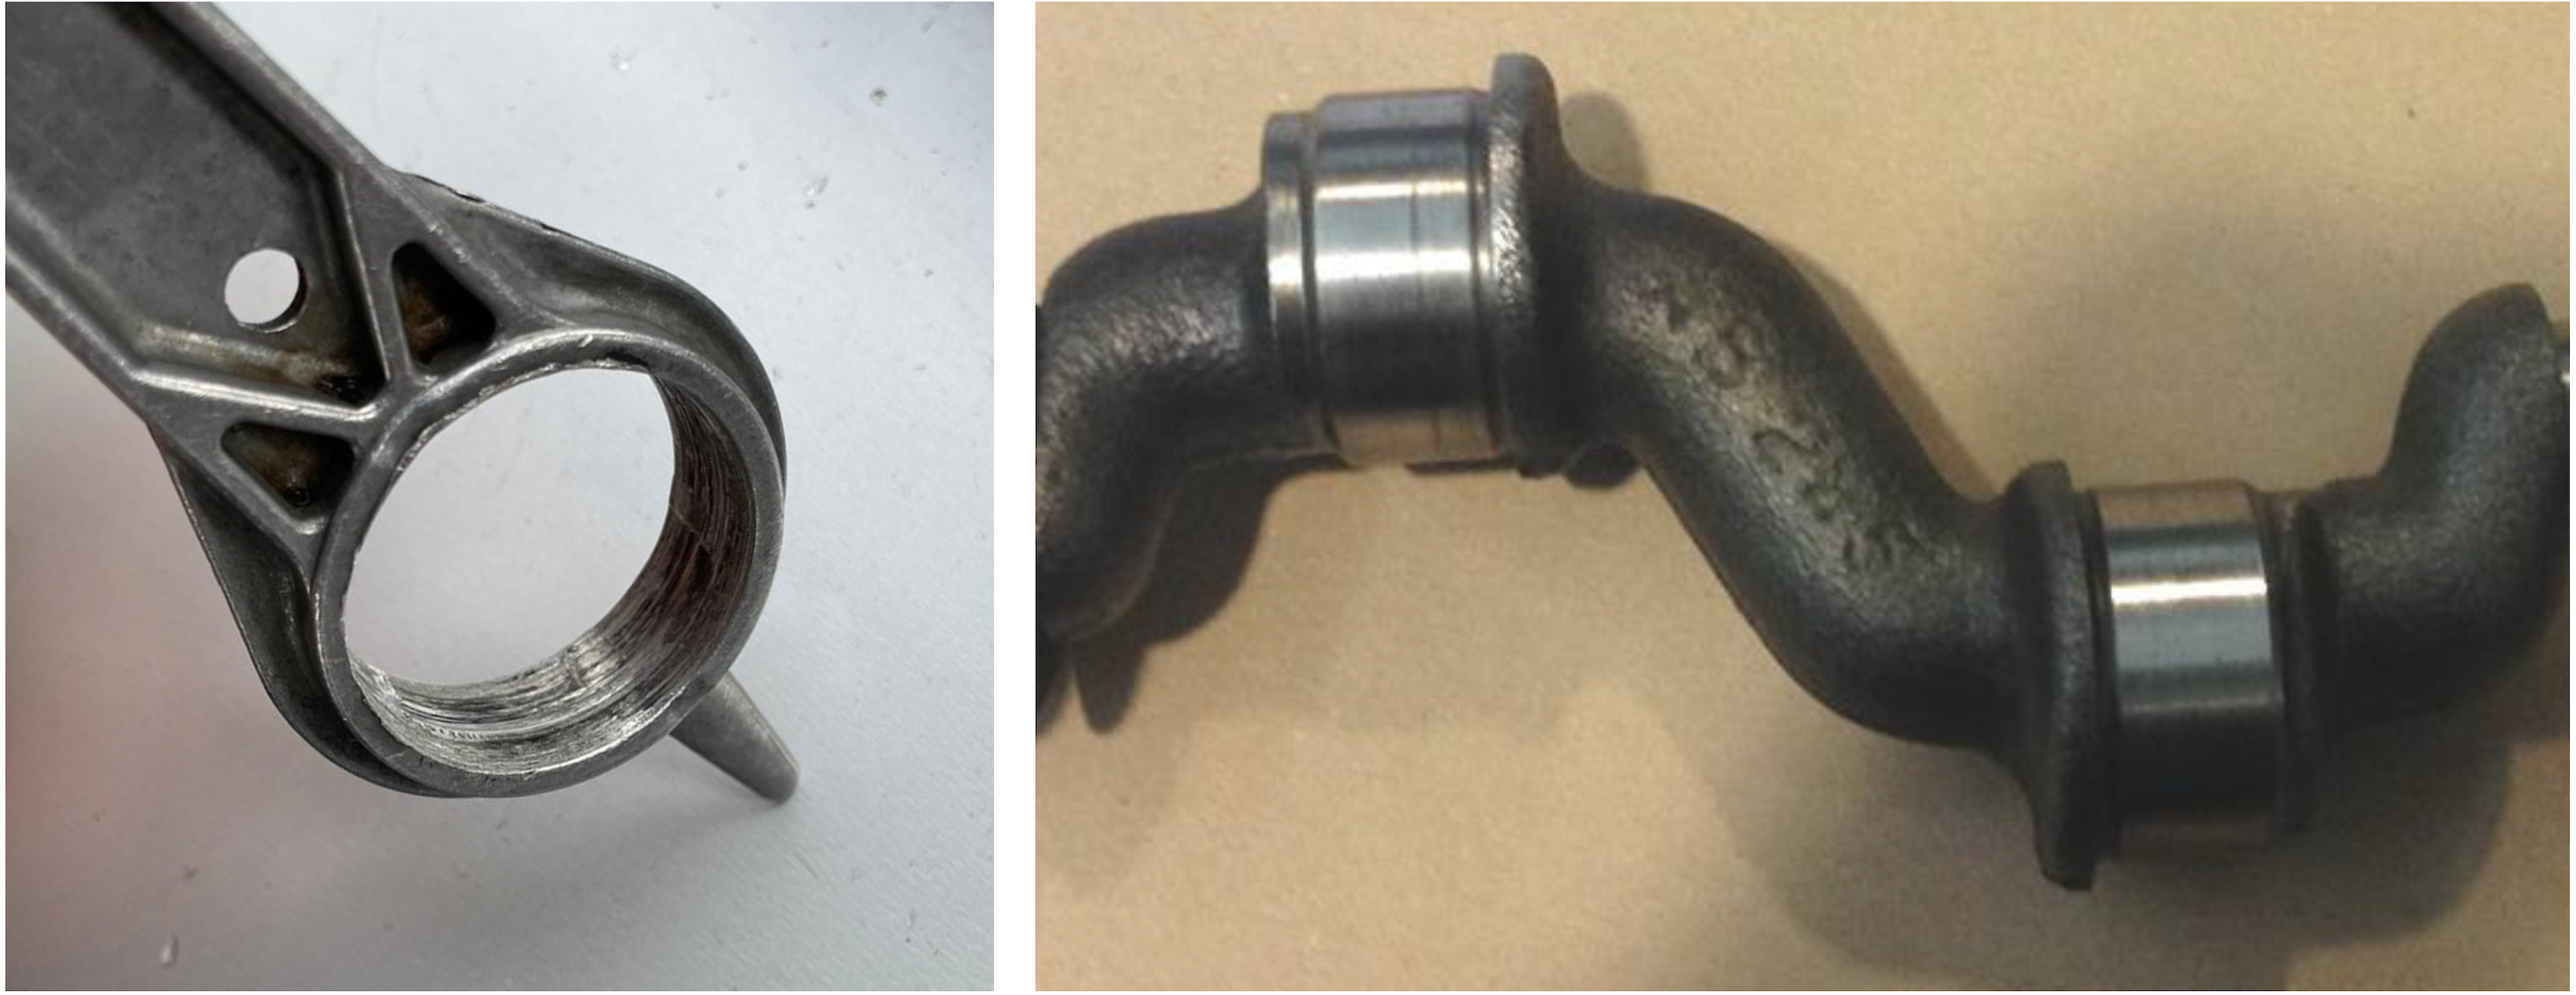
\includegraphics[scale=0.2]{Immagini/SuperficiBiellaManovella.png}
    \caption{Confronto superficie biella-manovella}
    \label{fig:SuperficiBiellaManovella}
\end{figure}

Questo fenomeno, in aggiunta ad una scarsa lubrificazione (dovuta a malfunzionamenti o ad un livello d’olio eccessivamente basso nel carter), può portare a problemi di maggiore rilievo come malfunzionamenti o rotture (sbiellamento), innescando una serie di problematiche che si amplificano reciprocamente.\\
Come si può notare dalla biella in esame, la compresenza di microerosione e lubrificazione inefficiente ha comportato la parziale ostruzione del condotto d’incanalamento dell’olio su tale superficie, generando a sua volta un peggioramento della lubrificazione e una maggiore criticità delle pressioni di contatto. Questo processo sfocerà quindi in perdite di rendimento, rumorosità e, qualora si protragga nel tempo, anche in danneggiamenti della macchina operatrice stessa.\\
\\
La biella in Fig.\ref{fig:DettaglioBiella} è difatti evidentemente storta a causa di un possibile principio di grippaggio, che tuttavia non ne ha comportato la rottura.
\begin{figure}[h]
    \centering
    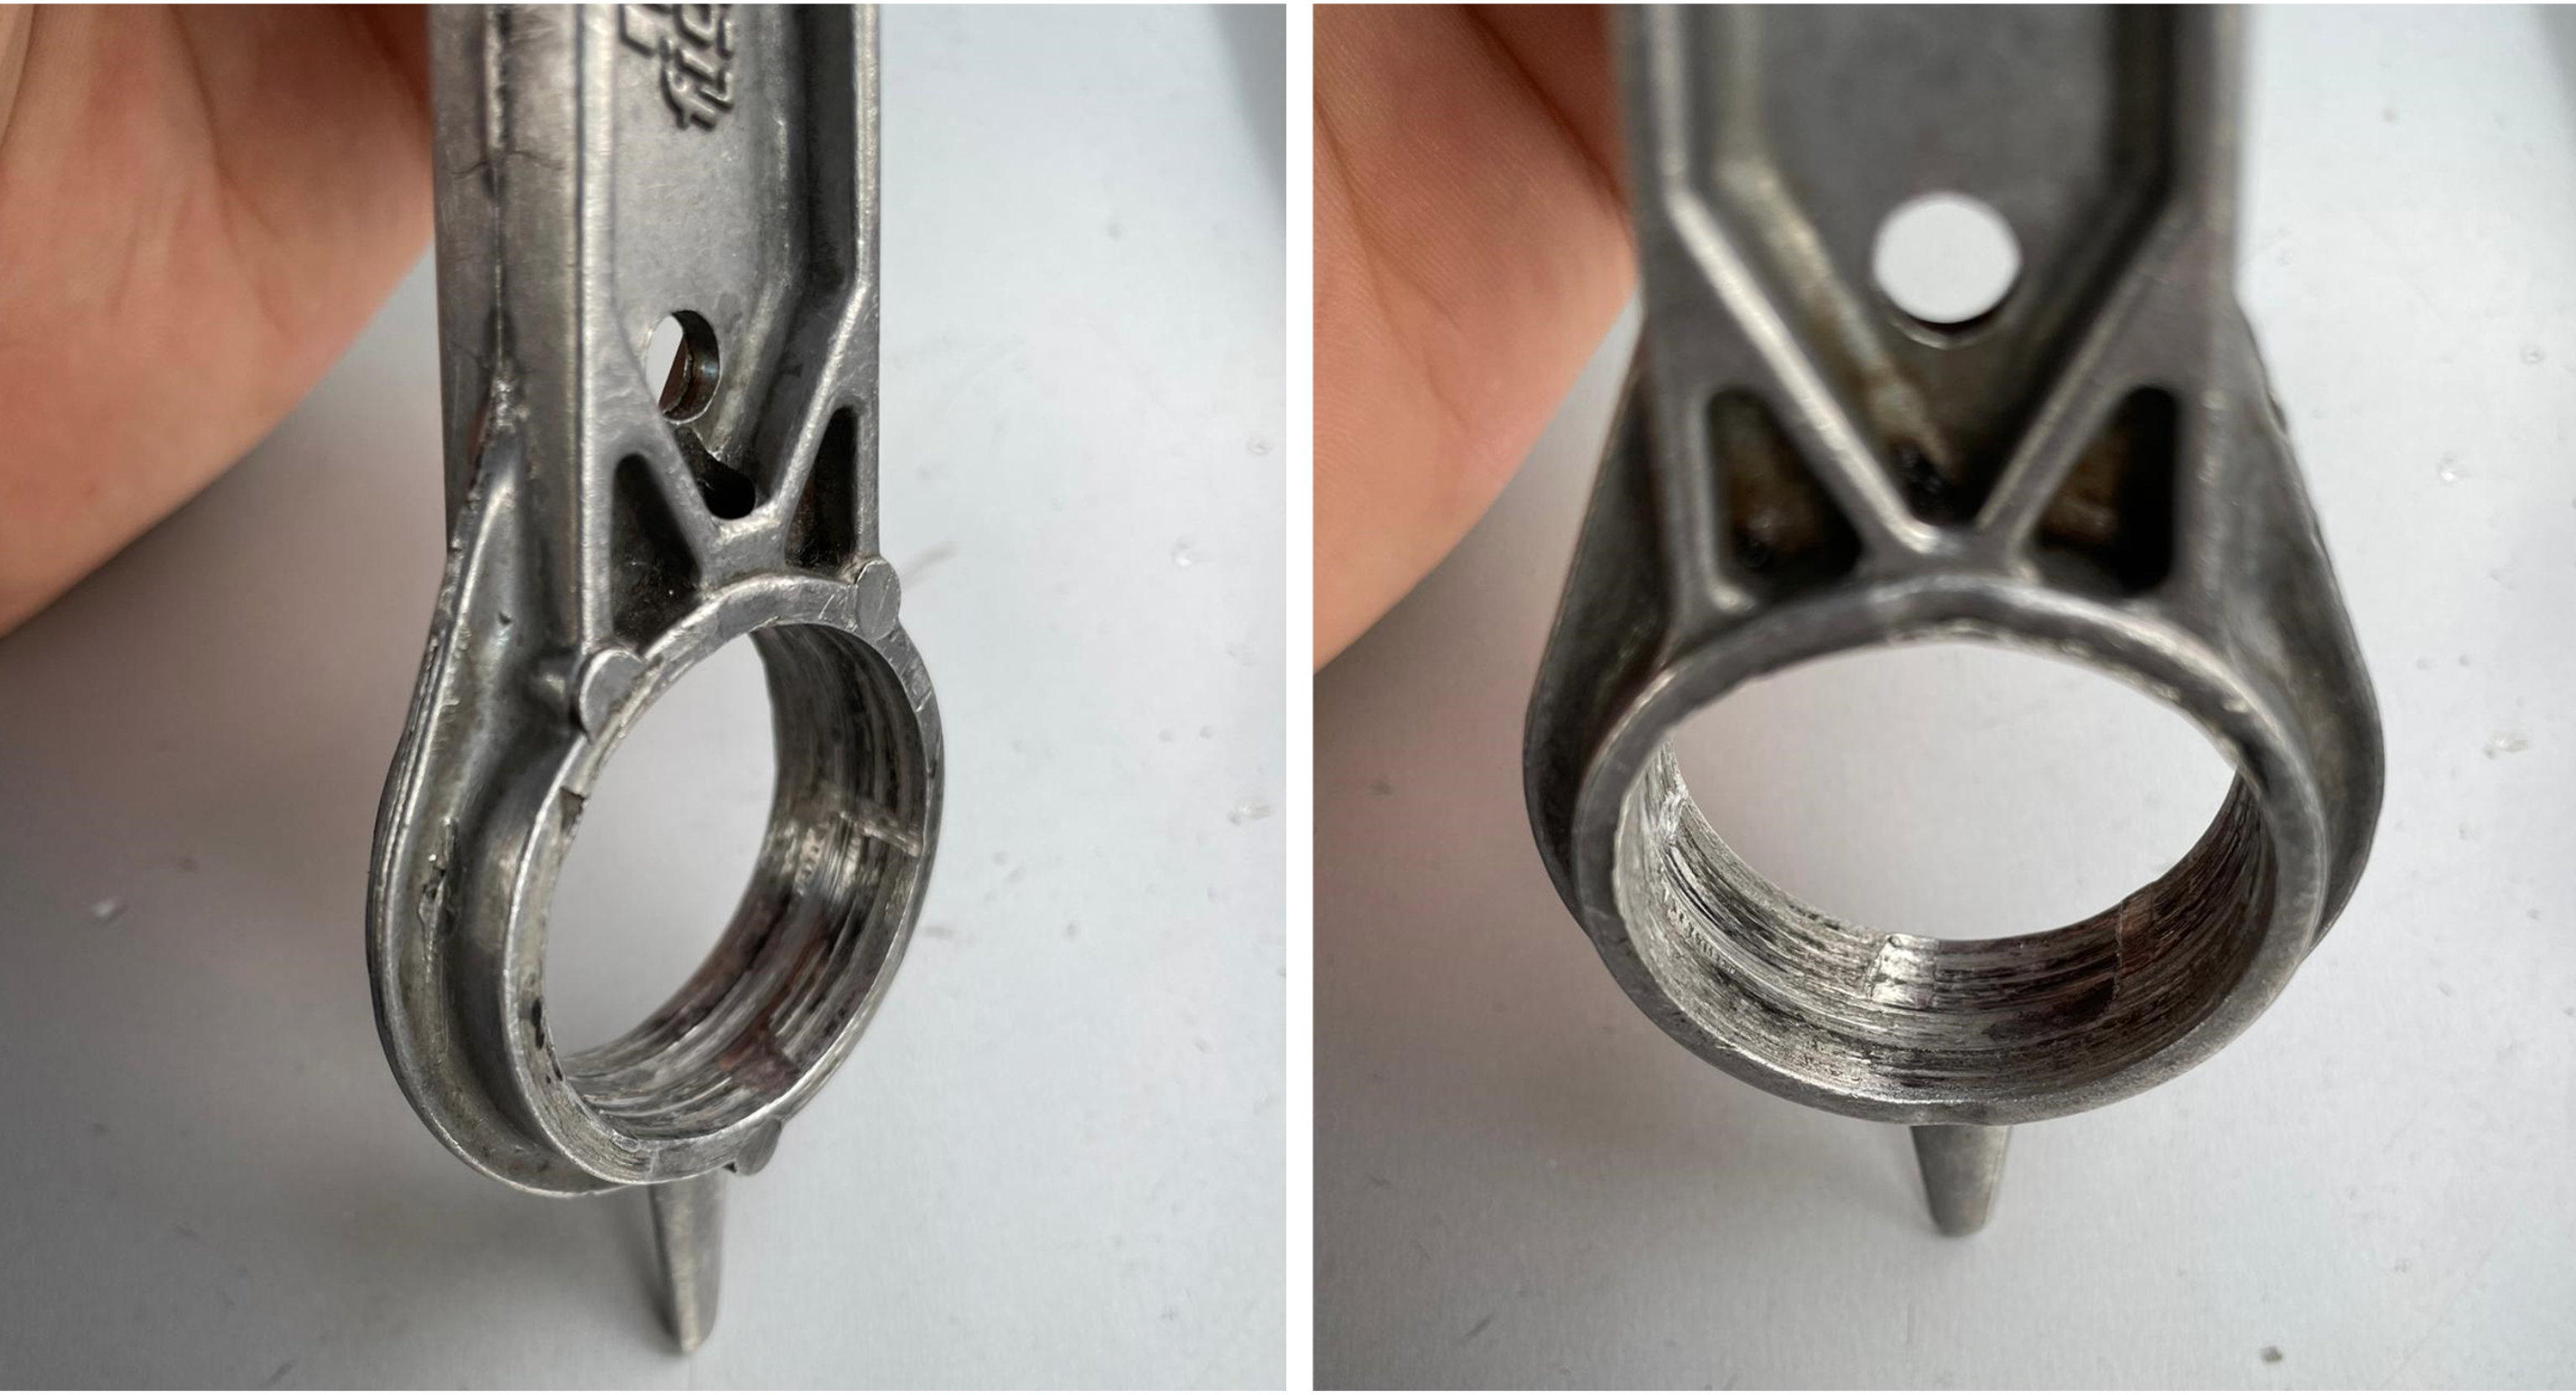
\includegraphics[scale=0.2]{Immagini/DettaglioBiella.png}
    \caption{Dettaglio biella}
    \label{fig:DettaglioBiella}
\end{figure}

Ben diversa è invece la condizione della biella appartenente ad un compressore alternativo Fiac ab 200-480 della medesima casa produttrice, ma con dimensioni e potenze superiori. In questo caso difatti i problemi citati precedentemente hanno comportato, dopo parecchie ore di servizio, la rottura totale di entrambe le bielle in seguito ad un violento grippaggio, in Fig.\ref{fig:Sbiellamento} .  
\begin{figure}[h]
    \centering
    \includegraphics[scale=0.35]{Immagini/Sbiellamento.png}
    \caption{Rottura biella}
    \label{fig:Sbiellamento}
\end{figure}
\newpage
\subsection{Manutenzione del compressore}
Per evitare le problematiche citate nel paragrafo precedente è opportuno eseguire periodicamente specifiche azioni di manutenzione sul compressore, in modo da garantirne un funzionamento ottimale ed una lunga durata di servizio. \begin{figure}[h]
    \centering
    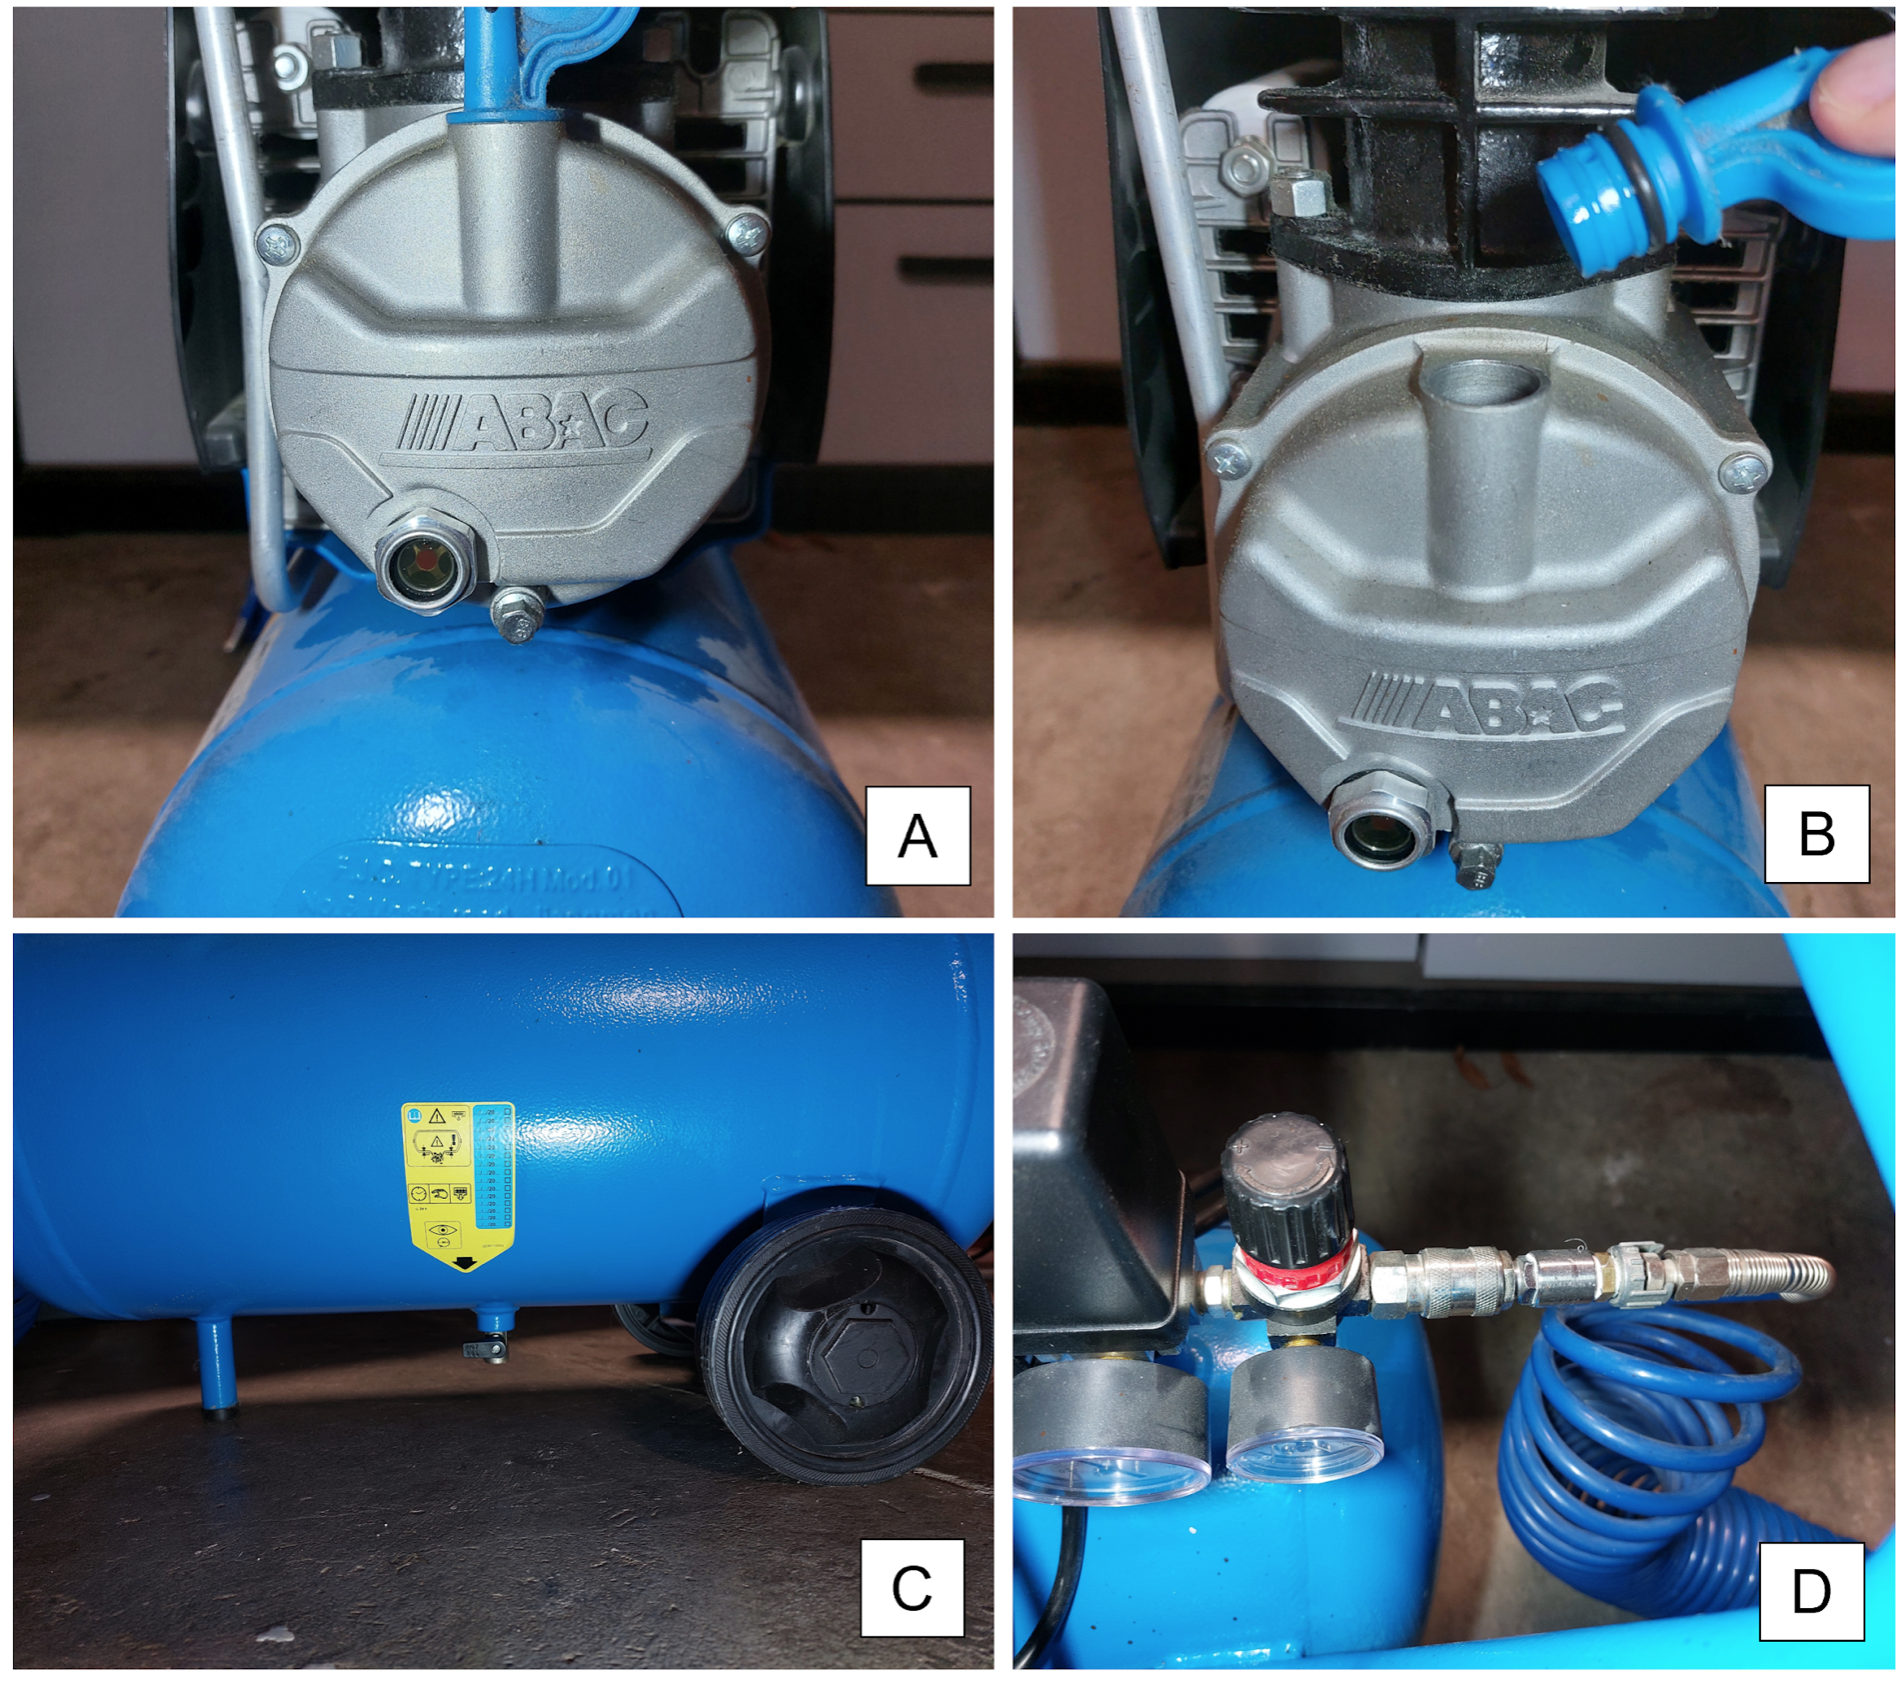
\includegraphics[scale=0.3]{Immagini/Manutenzione.png}
    \caption{Manutenzione del compressore}
    \label{fig:Manutenzione}
\end{figure}

Di seguito sono elencate le principali operazioni da effettuare sul dispositivo per eseguirne la corretta manutenzione:
\begin{itemize}
    \item CONTROLLO LIVELLO DELL’OLIO: Controllo periodico del livello d’olio nel carter del compressore, effettuato visivamente mediante l’apposito dado presente nella parte bassa del gruppo di pressurizzazione. Questo, infatti, presenta una parte centrale di vetro che consente di percepire la quantità di lubrificante all’interno del basamento (Fig.\ref{fig:Manutenzione}.a). \\
    Qualora il livello dell’olio sia più basso della sommità del dado sarà necessario verificare la presenza di possibili perdite ed eventualmente procedere con un rabbocco.
    \item RABBOCCO DELL’OLIO: Qualora il livello d’olio nel carter risulti essere troppo basso e si sia verificata l’assenza di perdite, si procede con l’aggiunta di lubrificante mediante l’apposito foro di rabbocco evidenziato in Fig.\ref{fig:Manutenzione}.b. L’olio aggiunto al sistema deve necessariamente rispettare gli standard qualitativi e le caratteristiche indicate dalla casa produttrice. 
    \item SCARICO DELLE CONDENSE DI SERBATOIO: È necessario eseguire periodicamente (una volta all’anno) lo scarico delle condense e dell’olio che potrebbero essersi accumulati all’interno del serbatoio durante il funzionamento del compressore.\\
    Si esegue mediante l’apertura graduale della valvola dedicata presente sotto al serbatoio (Fig.\ref{fig:Manutenzione}.c).
    \item CONTROLLO TENUTE LINEA DI MANDATA: Se con il serbatoio ad alte pressurizzazioni si percepiscono sfiati o fuoriuscite di fluido sarà opportuno verificare la tenuta degli elementi pneumatici installati sulla linea di mandata. \\
    Con il passare degli anni di servizio è comune un deterioramento dei nastri di tenuta in teflon (PTFE) con cui sono spesso collegati i vari dispositivi (Fig.\ref{fig:Manutenzione}.d). Qualora invece la perdita dovesse provenire da elementi più importanti come pressostato o valvola regolatrice sarà indispensabile sostituire il componente.
\end{itemize}
